\section{Introduction}

\textit{Schubert polynomials} were introduced by Lascoux and Sch\"utzenberger \cite{LS82a} as canonical representatives for Schubert cycles in the cohomology ring of the complete flag variety $\mathcal{F}\ell(n)$, which can be identified with a quotient of the polynomial ring $\Z[x_1,\dots,x_n]$ by the ideal generated by symmetric polynomials with no constant term.
In particular, given a permutation $w\in S_n$, the Schubert polynomial $\fk S_w(x)$ represents the cohomology class of the corresponding Schubert variety $X_w$.

There has been recent interest in establishing bounds for the \textit{principal specialization} $\nu_w := \fk S_w(1,\dots,1) \in \Z_{\geq0}$, which is known to give the degree of the matrix Schubert variety corresponding to $w$ \cite{KM05}.
The first result in this vein came from Weigandt \cite{Wei18} who showed that $\nu_w \geq 1 + p_{132}(w)$ where, in general, $p_u(w)$ represents the number of occurrences of the permutation pattern $u$ in $w$ (i.e. the number of subwords of $w$ whose entries appear in the same relative order as $u$).
This confirmed a conjecture of Stanley \cite{Sta17}, who believed that $\nu_w = 2$ if and only if $p_{132}(w)=1$.

Subsequently, Yibo Gao \cite{Gao21} improved this lower bound by showing that we can include the number of occurrences of $1432$ patterns in $w$, that is, $\nu_w \geq 1 + p_{132}(w) + p_{1432}(w)$.
In the same paper, Gao conjectured that there might be a way to include every permutation pattern in a lower bound for $\nu_w$.
Precisely, define the following sequence of coefficients $c_w$ indexed by permutations $w$ recursively:
\begin{enumerate}
    \item Set $c_\varnothing := 1$ (here $\varnothing$ is the unique permutation of size $0$).
    \item Assuming that $c_u$ has been defined for all permutations $u$ of size less than $n$, for $w\in S_n$ set \[
        c_w := \nu_w - \sum_{u< w} c_up_u(w)
    \] where this sum is taken over all permutation patterns $u$ properly contained in $w$ (so $u\neq w$).
\end{enumerate}

\begin{conjecture}[Gao\footnote{
    Gao remarks that Conjecture \ref{conj:gao} was also observed independently by Christian Gaetz.
} \cite{Gao21}]
\label{conj:gao}
    For all permutations $w$, $c_w\geq 0$.
\end{conjecture}

Note that if Conjecture $\ref{conj:gao}$ were true, then we would get a lower bound \[
    \nu_w \geq \sum_{u<w} c_up_u(w)
\]
with equality exactly when $c_w = 0$.
Since $c_\varnothing = c_{132} = c_{1432} = 1$ are the only nonzero values of $c_w$ for permutations $w$ of size $n\leq 4$, this would extend the previous bounds of Weigandt and Gao.

Conjecture \ref{conj:gao} has been checked empirically to hold for all permutations $w\in S_n$ for $n\leq 8$ \cite{Gao21}.
As more evidence, M\'esz\'aros and Tanjaya \cite{MT22} showed that Conjecture \ref{conj:gao} is true whenever $w$ avoids both of the patterns $1432$ and $1423$.

In this paper, we prove Conjecture \ref{conj:gao} for permutations $w$ that do not contain the pattern $1243$.
\begin{theorem}
\label{thm:gao_1243}
    For all $1243$-avoiding permutations $w$,
    $c_w\geq 0$.
\end{theorem}
We briefly outline the proof of Theorem \ref{thm:gao_1243}.
It is known that $\nu_w$ enumerates a collection of diagrams corresponding to $w$ called \textit{reduced bumpless pipe dreams} \cite{LLS21}.
To each of $w$'s reduced BPDs, we assign both a subword $v$ of $w$ and another reduced BPD corresponding to the permutation pattern $u$ that $v$ is an occurrence of in $w$.
Fixing $v$,
this gives an injection from the reduced BPDs of $w$ assigned to $v$ into a certain subset of \textit{minimal} reduced BPDs of $u$.
This is bijective when $w$ avoids the pattern $1243$, in which case $c_w$ will enumerate the set of minimal reduced bumpless pipe dreams for $w$ and Theorem \ref{thm:gao_1243} will follow.
In general, this yields an upper bound for the principal specialization $\nu_w$ in terms the minimal reduced BPDs of its permutation patterns (Corollary \ref{cor:schub_ub}).

In parallel, we will consider the \textit{$\beta$-Grothendieck polynomials} $\fk G^{(\beta)}_w(x)$ of Fomin and Kirillov \cite{FK94},
which specialize to Schubert polynomials in the case $\beta = 0$.
$\beta$-Grothendieck polynomials are known \cite{Hud14} to represent Schubert classes in the connective $K$-theory of the complete flag variety.
We can set up the same machinery for principal specializations of $\beta$-Grothendieck polynomials $\nu^{(\beta)}_w := \fk G^{(\beta)}_w(1,\dots,1)$,
which in this case are polynomials in $\Z_{\geq 0}[\beta]$,
by defining coefficients $c^{(\beta)}_w\in \Z[\beta]$ recursively as before:
\begin{enumerate}
    \item Set $c^{(\beta)}_\varnothing := 1$.
    \item Assuming that $c^{(\beta)}_u$ has been defined for all permutations $u$ of size less than $n$, for $w\in S_n$ set \[
        c^{(\beta)}_w :=
        \nu^{(\beta)}_w - \sum_{u<w} c^{(\beta)}_u p_u(w).
    \]
\end{enumerate}

Recall that a permutation is \textit{vexillary} if it avoids the pattern $2143$.
The techniques used to prove Theorem \ref{thm:gao_1243} are also applicable in the Grothendieck setting by restricting our view to a smaller pattern-avoidance class of permutations.
\begin{theorem}
\label{thm:groth_gao_1243_2143}
    For all vexillary $1243$-avoiding permutations $w$,
    $c^{(\beta)}_w \in \Z_{\geq0}[\beta]$.
\end{theorem}

The coefficients of $c^{(\beta)}_w$ have been verified by computer to be nonnegative for all permutations $w\in S_n$ of size $n\leq 9$.
This, coupled with the establishment of Theorem \ref{thm:groth_gao_1243_2143},
inspires us to make the following analogue of Conjecture \ref{conj:gao}.
\begin{conjecture}
\label{conj:groth_gao}
    For all permutations $w$, $c^{(\beta)}_w \in \Z_{\geq0}[\beta]$.
\end{conjecture}
We remark that $\nu_w$ and $c_w$ are just the constant terms of $\nu^{(\beta)}_w$ and $c^{(\beta)}_w$, respectively, so Conjecture \ref{conj:groth_gao} is a strengthening of Conjecture \ref{conj:gao}.





\section{Background \& definitions}

\subsection{Pattern containment}
\label{sect:pat}

Let $S_n$ denote the set of permutations on the set $[n] := \{1,2,\dots,n\}$.
We will write permutations as words in one-line notation.
In other words, for $w\in S_n$ a permutation, we identify $w$ with the word $w(1)w(2)\dots w(n)$.
Write $\abs*{w} := n$ for the size of $w$.

By a \textit{subword} $v$ of a permutation $w\in S_n$, we mean a map $v\colon [m]\to [n]$ obtained as a composition $[m]\to [n]\overset w\to [n]$ such that the first map is strictly increasing.
As with permutations, we will write $v = v(1)v(2)\cdots v(m)$ and $\abs*{v} := m$ for the size of $v$.
We use the relation $v\sseq w$ to denote that $v$ is a subword of $w$, whereas $v\subset w$ will denote the same with the additional constraint $v\neq w$.
This notation is suggestive in that we can think of $v$ as a subset of the inputs of $w$.

Let $w\in S_n$ be a permutation and let 
$v\sseq w$ be a subword of size $m$.
Define $\perm(v)$ to be the permutation $u\in S_m$ whose entries appear in the same relative order as the entries of $v$ i.e. $v(i) \leq v(j)$ if and only if $u(i) \leq u(j)$ for all $i,j\in [m]$.
As an example, the subword $253$ of $12453$ has $\perm(253) = 132$ since $2<3<5$.

Given two permutations $w\in S_n$ and $u\in S_m$,
we define $p_u(w)$ to be the number of subwords $v\sseq w$ satisfying $\perm(v) = u$.
We say that $w$ \textit{avoids the pattern} $u$, or is \textit{$u$-avoiding}, if $p_u(w) = 0$.
Otherwise we say that $w$ \textit{contains the pattern} $u$.

Continuing our example, $p_{132}(12453) = 4$ (the occurrences are $143$, $153$, $243$, and $253$), so $12453$ contains the pattern $132$, even though $132$ is not a \textit{subword} of $12453$.
On the other hand, $12453$ avoids the pattern $2143$ since $p_{2143}(12453) = 0$.

Permutations that are $2143$-avoiding have a special name; they are known as \textit{vexillary} permutations.

We will use the notation $u\leq w$ to denote that $w$ contains the pattern $u$ and the notation $u< w$ to additionally indicate that $u\neq w$.\footnote{
    This is not to be confused with the \textit{Bruhat order} on $S_n$, which is also often denoted by $\leq$.
}
It is important to make the distinction between the partial orders $\sseq$, which is defined on \textit{subwords} of $w$, and $\leq$, which is defined on \textit{permutations} that appear as a pattern in $w$.

By convention, we define $[0]$ to be empty and let $\varnothing$ denote the unique permutation in $S_0$.
Every permutation $w$ contains $\varnothing$ as a pattern precisely once, that is $p_\varnothing(w) = 1$, and the occurrence of this pattern will also be denoted $\varnothing$.

We remark that the permutation statistics given by the pattern count functions $p_u$ are interesting in their own right.
As an example, $p_{21}(w)$ counts the number of \textit{inversions} in $w$, which are pairs of indices $(i,j)$ satisfying $i<j$ and $w(i)>w(j)$.
This quantity is called the \textit{\textup{(}Coxeter\textup{)} length} of $w$, which we denote by $\ell(w) := p_{21}(w)$.



\subsection{Bumpless pipe dreams and alternating sign matrices}
\label{sect:bpd}

A \textit{bumpless pipe dream} of size $n$ is a filling of the $n\times n$ grid using the tiles \[
    \bigblank\quad
    \bighorizontal\quad
    \bigvertical\quad
    \bigcross\quad
    \bigrelbow\quad
    \bigjelbow
\] such that the resulting configuration is a network consisting of $n$ ``pipes,'' each entering from a column along the south edge of the grid and exiting through a row along the east edge \cite{LLS21, Wei21}.
In order from left-to-right, we will refer to these tiles as the \textit{blank}, \textit{horizontal}, \textit{vertical}, \textit{cross}, \textit{r-elbow}, and \textit{j-elbow}, respectively.

\begin{figure}[ht]
    \begin{tikzpicture}[scale=0.5]
    \drawBPDwithL{0}{0}{7}{
        0,0,0,0,4,2,2,
        0,0,4,2,3,2,2,
        0,0,1,0,1,4,2,
        0,0,1,4,3,3,2,
        0,4,3,3,5,1,4,
        4,3,5,1,4,3,3,
        1,1,4,3,3,3,3
    }{1/2,2/1,3/6,4/4,5/7,6/5,7/3}

    \begin{scope}[shift={(10,0)}]
    \drawBPDwithL{0}{0}{7}{
        0,4,2,2,2,2,2,
        0,1,0,4,2,2,2,
        0,1,4,5,4,2,2,
        0,1,1,0,1,4,2,
        4,3,3,2,3,3,2,
        1,1,1,4,5,1,4,
        1,1,1,1,4,3,3
    }{1/2,2/3,3/4,4/6,5/1,6/7,7/5}
    \end{scope}
    \end{tikzpicture}
    
    \caption{Two bumpless pipe dreams of size $7$.}
    \label{fig:bpd}
\end{figure}

We let $\BPD(n)$ denote the collection of bumpless pipe dreams of size $n$.
The standard convention is to plot each $B\in \BPD(n)$ using matrix coordinates.
Write $B_{i,j}$ for the tile in $B$ that is at position $(i,j)$.
We use the notation $B(\blank)$ for the set of positions $(i,j)$ such that $B_{i,j} = \blank$
(and we make analogous definitions for $\horizontal$, $\vertical$, $\cross$, $\relbow$, and $\jelbow$).

We now make a brief digression to discuss a connection between bumpless pipe dreams and a related combinatorial object.
An \textit{alternating sign matrix} of size $n$ is a square $n\times n$ matrix $A$ consisting of the entries $0$, $+1$, and $-1$ such that in each row and column of $A$, the entries sum to $+1$ with the nonzero entries alternating in sign.
These conditions imply that each row and column of $A$ has at least one nonzero entry with the initial and final nonzero entries always being $+1$'s.
Let $\ASM(n)$ denote the set of alternating sign matrices of size $n$.

There is a bijection $\Phi\colon \BPD(n) \to \ASM(n)$ \cite{Wei21},
where for $B$ a bumpless pipe dream of size $n$, we get an $n\times n$ alternating sign matrix via the formula \[
    \Phi(B)_{i,j} := \begin{cases}
        +1 & B_{i,j} = $\relbow$, \\
        -1 & B_{i,j} = $\jelbow$, \\
        0 & \text{else.}
    \end{cases}
\]
This means that the elbows in each row and each column of $B$ are alternating between $\relbow$ and $\jelbow$ with the initial and final elbows always being $\relbow$'s.
It is often helpful to have this alternative view of bumpless pipe dreams.

\begin{figure}
    \centering
    \[\begin{pmatrix}
     0& 0& 0& 0&+1& 0& 0\\
     0& 0&+1& 0& 0& 0& 0\\
     0& 0& 0& 0& 0&+1& 0\\
     0& 0& 0&+1& 0& 0& 0\\
     0&+1& 0& 0&-1& 0&+1\\
    +1& 0&-1& 0&+1& 0& 0\\
     0& 0&+1& 0& 0& 0& 0
    \end{pmatrix}\]
    \caption{The alternating sign matrix $\Phi(B)$ corresponding to the first bumpless pipe dream $B$ in Figure \ref{fig:bpd}.}
    \label{fig:asm}
\end{figure}

We now return to our introduction of bumpless pipe dreams.
To each $B\in \BPD(n)$, we can assign a permutation $w(B)\in S_n$ by setting $w(B)(x) := y$ if and only if $y\to x$ is a pipe in $B$ (that is, the pipe in $B$ entering from column $y$ exits in row $x$).
We call $w(B)$ the \textit{wiring} of the bumpless pipe dream $B$.
The bumpless pipe dreams in Figure \ref{fig:bpd} have wirings $2164753$ and $2346175$, respectively.
Write $\mbox{Wires}(w)$ for set of bumpless pipe dreams that have wiring $w$.

There is an alternative way to interpret how the network of pipes in $B$ behaves at crosses; namely, two pipes will cross only at the first $\cross$ they partake in, otherwise diverging away from each other at subsequent crosses.
To make this precise, totally order $B(\cross)$ first by rows from bottom-to-top, then within each row from left-to-right.
We now modify $B$ as follows:
for each $(i,j)\in B(\cross)$ in the prescribed order, check if the pipes passing through $(i,j)$ also cross at another position southwest of $(i,j)$.
If they do, change the tile at $(i,j)$ from a cross to a \textit{bump}:\footnote{
    This eponymous tile, absent in the bumpless pipe dream model, is present in the older \textit{pipe dream} model.
} \[
    \bigcross\quad
    \raisebox{4pt}{$\longmapsto$}\quad
    \bigbump
\]
Let $\reduce(B)$ denote the diagram obtained by this process.
See Figure \ref{fig:bpd_K} for an example.

\begin{figure}
    \centering
    \begin{tikzpicture}[scale=0.5]
    \drawBPDwithL{0}{0}{7}{
        0,0,0,0,4,2,2,
        0,0,4,2,3,2,2,
        0,0,1,0,1,4,2,
        0,0,1,4,3,3,2,
        0,4,3,3,5,1,4,
        4,3,5,1,4,3,3,
        1,1,4,3,3,3,3
    }{1/2,2/1,3/6,4/4,5/7,6/5,7/3}
    \node at (9,-3) {$\longmapsto$};
    \drawBPDwithL{11}{0}{7}{
        0,0,0,0,4,2,2,
        0,0,4,2,3,2,2,
        0,0,1,0,1,4,2,
        0,0,1,4,6,3,2,
        0,4,6,3,5,1,4,
        4,3,5,1,4,3,3,
        1,1,4,3,3,3,3
    }{1/4,2/2,3/6,4/1,5/7,6/5,7/3}
    \end{tikzpicture}

    
    \caption{The resulting network of pipes $\reduce(B)$ obtained from the first bumpless pipe dream $B$ in Figure \ref{fig:bpd}.}
    \label{fig:bpd_K}
\end{figure}

We get another permutation in $S_n$ associated to $B$, denoted $\partial(B)$, by setting $\partial(B)(x) := y$ if and only if $y\to x$ is a pipe appearing in $\reduce(B)$.
It turns out that this is the more natural permutation to attach to $B$, so we call $\partial(B)$ \underline{the} \textit{permutation} of $B$.
Keeping with our example, the first bumpless pipe dream in Figure \ref{fig:bpd} has permutation $4261753$, as shown in Figure \ref{fig:bpd_K}.
The second BPD in Figure \ref{fig:bpd} has no double crossings between its pipes and hence remains unchanged by this process, so it has permutation $2356175$.
Let $\BPD(w)$ denote the set of bumpless pipe dreams with permutation $w$.

We say that a bumpless pipe dream is \textit{reduced} if no two of its pipes cross more than once.
A bumpless pipe dream $B$ is reduced if and only if $\reduce(B) = B$, and in this case the wiring of $B$ and the permutation of $B$ coincide.
In Figure \ref{fig:bpd}, the second BPD is reduced while the first is not.
Write $\BPD_0(n)$ for the set of reduced bumpless pipe dreams of size $n$.
For $w\in S_n$, we also write $\BPD_0(w) = \BPD(w)\cap \BPD_0(n)$ for the set of reduced BPDs with permutation $w$.
Notice that equivalently $\BPD_0(w) = \Wires(w)\cap \BPD_0(n)$.

There is a unique bumpless pipe dream of size $0$ which is reduced and has permutation $\varnothing$.
We also use the symbol $\varnothing$ to denote this bumpless pipe dream.

\begin{figure}
    \begin{tikzpicture}[scale=0.5]
    \drawBPDwithL{0}{0}{4}{
        4,2,2,2,
        1,4,2,2,
        1,1,0,4,
        1,1,4,3
    }{1/1,2/2,3/4,4/3}
    
    \drawBPDwithL{6}{0}{4}{
        4,2,2,2,
        1,0,4,2,
        1,4,5,4,
        1,1,4,3
    }{1/1,2/2,3/4,4/3}
    
    \drawBPDwithL{12}{0}{4}{
        0,4,2,2,
        4,5,4,2,
        1,4,5,4,
        1,1,4,3
    }{1/1,2/2,3/4,4/3}

    \draw[dotted] (18,0.5) -- (18,-4.5);
    
    \drawBPDwithL{20}{0}{4}{
        0,0,4,2,
        0,4,3,2,
        4,3,5,4,
        1,1,4,3
    }{1/1,2/2,3/4,4/3}
    \end{tikzpicture}


    
    \caption{The four bumpless pipe dreams in $\Wires(1243)$.
    The three on the left are reduced and form $\BPD_0(1243) = \BPD(1243)$, while the one on the right is not.}
    \label{fig:red_bpd}
\end{figure}



\subsection{Grothendieck and Schubert polynomials}
\label{sect:polys}

Throughout this subsection, fix a permutation $w\in S_n$.

The \textit{$\beta$-Grothendieck polynomial} for $w$ is a polynomial in $\Z_{\geq0}[\beta][x_1,x_2,\dots]$ which we will define as the generating function \begin{equation}
\label{eq:groth}
    \fk G^{(\beta)}_w(x_1,\dots,x_{n-1}) :=
    \sum_{B\in \BPD(w)}
    \beta^{-\ell(w)}
    \bigg(
        \prod_{(i,j)\in B(\smallblank)} \beta x_i
    \bigg)
    \bigg(
        \prod_{(i,j)\in B(\smalljelbow)} (1+\beta x_i)
    \bigg).
\end{equation}
It is known that $\abs*{B(\blank)} \geq \ell(w)$ with equality if and only if $B$ is reduced \cite{Wei21},
so $\fk G^{(\beta)}_w(x)$ is indeed a polynomial in $\Z_{\geq 0}[\beta][x_1,x_2,\dots]$.

We compute the $\beta$-Grothendieck polynomial for $w = 1243$ as an example.
The 3 bumpless pipe dreams for in $\BPD(1243)$ are illustrated in Figure \ref{fig:red_bpd}.
Hence $\fk G_{1243}^{(\beta)}(x_1,x_2,x_3) = x_3 + x_2(1+\beta x_3) + x_1(1+\beta x_2)(1+\beta x_3) = x_1+x_2+x_3 + \beta(x_1x_2 + x_1x_3 + x_2x_3) + \beta^2x_1x_2x_3$.

$\beta$-Grothendieck polynomials were originally introduced by Fomin and Kirillov \cite{FK94} to study solutions to the Yang--Baxter equation.
The above formulation comes from work of Lascoux \cite{Las02} which was later translated by Weigandt \cite{Wei21} using the language of bumpless pipe dreams.

Of interest to us is the \textit{principal specialization} of the $\beta$-Grothendieck polynomial $\nu_w^{(\beta)} := \fk G_w^{(\beta)}(1,\dots,1)$, which itself is a polynomial in $\Z_{\geq 0}[\beta]$.
From the above, $\nu^{(\beta)}_w$ can be calculated as \[
    \nu^{(\beta)}_w = \fk G^{(\beta)}_w(1,\dots,1) =
    \sum_{B\in \BPD(w)}
    \beta^{\abs*{B(\smallblank)}-\ell(w)}
    (1+\beta)^{\abs*{B(\smalljelbow)}}.
\]
Continuing our example above, we have $\nu_{1243}^{(\beta)} = 3 + 3\beta + \beta^2$.
To simplify notation, define the \textit{$\beta$-weight} of a bumpless pipe dream $B\in \BPD(w)$ to be the quantity $\wt^{(\beta)}(B) := \beta^{\abs*{B(\smallblank)}-\ell(w)} (1+\beta)^{\abs*{B(\smalljelbow)}} \in \Z_{\geq 0}[\beta]$.
Extend this weight to collections of bumpless pipe dreams $\mathcal S\sseq \BPD(n)$ by setting $\wt^{(\beta)}(\mathcal S) := \sum_{B\in \mathcal S} \wt^{(\beta)}(B)$.
Then $\nu^{(\beta)}_w = \wt^{(\beta)}(\BPD(w))$.

Let $B\in \BPD(w)$ be a bumpless pipe dream with permutation $w$.
The term contributed by $B$ in Equation \ref{eq:groth} has a factor of $\beta$ if and only if $\abs*{B(\blank)} > \ell(w)$, which, as we remarked, occurs exactly when $B$ is not reduced.
The polynomial $\fk S_w(x) := \fk G^{(0)}_w(x)$ obtained by specializing $\beta = 0$ is thus a generating function over reduced bumpless pipe dreams: \[
    \fk S_w(x_1,\dots,x_{n-1}) =
    \sum_{B\in \BPD_0(w)}
    \prod_{(i,j)\in B(\smallblank)} x_i.
\]
This is the \textit{Schubert polynomial} for $w$ of Lascoux and Sch\"utzenberger \cite{LS82a,LLS21}.
For example, the Schubert polynomial for $w = 1243$ is $\fk S_{1243}(x_1,x_2,x_3) = x_1+x_2+x_3$, the $\beta$-degree 0 component of $\fk G_{1243}^{(\beta)}$.
Writing $\nu_w := \nu^{(0)}_w$, we see that the principal specialization of the Schubert polynomial $\fk S_w(x)$ gives an enumeration \[
    \nu_w = \fk S_w(1,\dots,1) = \abs*{\BPD_0(w)}.
\]

We end this section with a few remarks.
The first is that there are other specializations of $\beta$ that appear in the literature.
Taking $\beta = -1$ recovers the (ordinary) Grothendieck polynomials $\fk G_w(x) = \fk G_w^{(-1)}(x)$ of Lascoux and Sch\"utzenberger \cite{LS82b}.
With $\beta = 1$, notice that the $1$-weight of a bumpless pipe dream $B\in \BPD(n)$ is simply $\wt^{(1)}(B) = 2^{\abs*{B(\smalljelbow)}}$.
This weight is interesting when considering the bijection to alternating sign matrices:
since the number of $\jelbow$'s in $B$ is the same as the number of $-1$'s in $\Phi(B)$, $\wt^{(1)}(B)$ is the same as the weight of $\Phi(B)$ in what is known as the \textit{$2$-enumeration} of $\ASM(n)$ \cite{EKLP92}.

It should also be noted that the specializations $\nu^{(\beta)}_w$ have previously been studied for $w$ vexillary, where a determinantal upper bound was established in terms of Delannoy paths on Young tableaux \cite{MPP22}.
There is a $q$-analog of $\nu^{(\beta)}_w$ given by $\fk G^{(\beta)}_w(1,q,q^2,\dots)$ where we instead send $x_i\mapsto q^{i-1}$.
Fomin and Stanley \cite{FS94} proved an elegant formula (originally conjectured by Macdonald \cite{Mac91}) which computes the Schubert $q$-analog principal specialization $\fk S_w(1,q,q^2,\dots)$ as a weighted sum over the reduced words for $w$.
This specializes to a formula for $\nu_w$ by taking $q=1$.
Marberg and Pawlowski \cite{MP21} proved an analogous formula for the $q$-specializations of \textit{back stable} Schubert and $\beta$-Grothendieck polynomials, which are power series variants of Schubert and $\beta$-Grothendieck polynomials that admit variables $x_i$ with indices $i\leq 0$.





\section{Main results}

\subsection{Removing pipes}
\label{sect:rem_pipes}

\begin{definition}
    Let $B\in \BPD(n)$.
    \begin{itemize}
        \item Say that a pipe $y\to x$ in $B$ is \textit{hook-shaped} if it only contains a single bend, which necessarily must occur at $(x,y)\in B(\relbow)$.
        \item Say that a pipe $y\to x$ in $B$ is \textit{removable} if it is hook-shaped, and $(x,y)$ is the only $\relbow$ occurring in row $x$ and in column $y$.
        \item Say that $B$ is \textit{minimal} if it contains no removable pipes.
    \end{itemize}
\end{definition}

In the language of alternating sign matrices, as a pipe $y\to x$ is removable in $B$ if and only if $\Phi(B)_{x,y} = +1$, and this is the only nonzero entry in row $x$ and column $y$ of $\Phi(B)$.

\begin{figure}
    \centering
    \begin{tikzpicture}[scale=0.5]
    \drawBPDwithRPL{0}{0}{7}{
        0,0,0,0,4,2,2,
        0,0,4,2,3,2,2,
        0,0,1,0,1,0,0,
        0,0,1,0,1,0,0,
        0,4,3,2,5,0,4,
        4,3,5,0,4,2,3,
        1,1,4,2,3,2,3
    }{3/6,4/4}{1/2,2/1,3/6,4/4,5/7,6/5,7/3}
    \drawBPDwithL{10}{0}{7}{
        0,0,0,0,4,2,2,
        0,0,0,4,3,2,2,
        0,0,4,5,1,4,2,
        0,0,1,4,3,3,2,
        0,4,3,3,5,1,4,
        4,3,5,1,4,3,3,
        1,1,4,3,3,3,3
    }{1/2,2/1,3/6,4/4,5/7,6/5,7/3}
    \end{tikzpicture}
    \caption{On the left, the first bumpless pipe dream from Figure \ref{fig:bpd} with its two removable pipes indicated via dashed lines.
    On the right, a similar BPD which is minimal.}
    \label{fig:min_bpd}
\end{figure}

Fix a permutation $w\in S_n$.
For $B\in \Wires(w)$ a BPD with (complete set of) removable pipes $y_1\to x_1,\dots,y_r\to x_r$, we get a subword $v\sseq w$ of size $n-r$ simply by ignoring the values $y_1,\dots,y_r$ in $w$.
For the BPD on the left in Figure \ref{fig:min_bpd}, this gives the subword $21753$ of $2164753$.
Let $\Wires(w;v)$ denote the collection of all $B\in \Wires(w)$ that correspond to the subword $v\sseq w$ in this way.
This gives a partition \[
    \Wires(w) = \bigsqcup_{v\sseq w} \Wires(w;v).
\]
In particular, $\Wires(w;w)$ is the set of minimal bumpless pipe dreams with wiring $w$.

Now, fix a subword $v\sseq w$ of size $m$ and write $u = \perm(v) \in S_m$.
Let $y_1\to x_1,\dots,y_r\to x_r$ denote the removable pipes in any bumpless pipe dream in $\Wires(w;v)$.
In other words, $r = n-m$, $y_1,\dots,y_r$ are the entries in $w$ not appearing in $v$, and $x_1,\dots,x_r$ are the corresponding indices.
Assume $y_1< \cdots< y_r$.
We also write $S = \{s_1<\cdots<s_m\} = [n]\sm \{x_1,\dots,x_r\}$ for the set of positions of $v$ as a subword in $w$ and $T = \{t_1<\cdots<t_m\} = [n]\sm \{y_1,\dots,y_r\}$ for the set of entries of $v$.
Note that this means $w(s_i) = v(i) = t_{u(i)}$ for all $i\in[m]$.

Let $B\in \Wires(w;v)$.
We now describe a procedure for removing the (suggestively named) removable pipes from $B$.
This will produce a minimal pipe dream $\minimize(B)\in \Wires(u;u)$.
The process is most easily described by viewing $B$ as its corresponding alternating sign matrix $\Phi(B)$.
In this setting, we simply take the $m\times m$ submatrix $\Phi(B)_{S,T}$ of $\Phi(B)$ on rows $S$ and columns $T$.
Since $\Phi(B)_{x_1,y_1},\dots,\Phi(B)_{x_r,y_r}$ are precisely the $+1$'s in $\Phi(B)$ with the property that they are the only nonzero entry in their row and column, the nonzero entries in each row of $\Phi(B)$ indexed by $S$ occur only in the columns indexed by $T$, and vice versa, so the property of being an ASM is preserved.

We now describe the map $B\mapsto \minimize(B)$ using bumpless pipe dreams.
We do this in three steps:
\begin{enumerate}
    \item Erase the pipes $y_1\to x_1,\dots,y_r\to x_r$ from $B$.
    \item Since each pipe $y_k\to x_k$ ($1\leq k\leq r$) was removable, the remaining tiles in row $x_k$ consist entirely of $\blank$ and $\vertical$ tiles.
    We can now \textit{contract} the rows $x_1,\dots,x_r$ whilst maintaining the connectivity of the pipes that pass through them
    (i.e. delete the cells in these rows from $B$ and then top-justify the resulting diagram).
    \item Likewise, the remaining tiles in each column $y_k$ ($1\leq k\leq r$) consist entirely of $\blank$ and $\horizontal$ tiles.
    We can now \textit{contract} the columns $y_1,\dots,y_r$ whilst maintaining the connectivity of the pipes that pass through them
    (i.e. delete the cells in these columns from $B$ and then left-justify the resulting diagram).
\end{enumerate}
See Figure \ref{fig:phi_v^w} for an example.
Note that $\minimize(B)_{i,j} = B_{s_i,t_j}$ for all $i,j\in[m]$.
Since all the wires remain connected, $\minimize(B)$ is a bumpless pipe dream which, in particular, is the bumpless pipe dream corresponding to the ASM $\Phi(B)_{S,T}$.

\begin{figure}
    \centering

    \begin{tikzpicture}[scale=0.38]
    \drawBPDwithRP{0}{0}{7}{
        0,0,0,0,4,2,2,
        0,0,4,2,3,2,2,
        0,0,1,0,1,0,0,
        0,0,1,0,1,0,0,
        0,4,3,2,5,0,4,
        4,3,5,0,4,2,3,
        1,1,4,2,3,2,3
    }{3/6,4/4}
    \filldraw[gray,opacity=0.3]
    (-0.5,-1.5) rectangle (6.5,-3.5)
    (2.5,0.5) rectangle (3.5,-6.5)
    (4.5,0.5) rectangle (5.5,-6.5);
    \node at (3,-7) {$y_1$};
    \node at (5,-7) {$y_2$};
    \node at (7.2,-2) {$x_1$};
    \node at (7.2,-3) {$x_2$};
    \node at (8.5,-3) {$\overset{(1)}\longrightarrow$};

    \begin{scope}[shift = {(10,0)}]
    \drawBPD{0}{0}{7}{
        0,0,0,0,4,2,2,
        0,0,4,2,3,2,2,
        0,0,1,0,1,0,0,
        0,0,1,0,1,0,0,
        0,4,3,2,5,0,4,
        4,3,5,0,4,2,3,
        1,1,4,2,3,2,3
    }
    \filldraw[gray,opacity=0.3]
    (-0.5,-1.5) rectangle (6.5,-3.5)
    (2.5,0.5) rectangle (3.5,-6.5)
    (4.5,0.5) rectangle (5.5,-6.5);
    \node at (7.5,-3) {$\overset{(2)}\longrightarrow$};
    \end{scope}

    \begin{scope}[shift = {(19,-1)}]
    \drawRectangleBPD{0}{0}{5}{7}{
        0,0,0,0,4,2,2,
        0,0,4,2,3,2,2,
        0,4,3,2,5,0,4,
        4,3,5,0,4,2,3,
        1,1,4,2,3,2,3
    }
    \filldraw[gray,opacity=0.3]
    (2.5,0.5) rectangle (3.5,-4.5)
    (4.5,0.5) rectangle (5.5,-4.5);
    \node at (7.5,-2) {$\overset{(3)}\longrightarrow$};
    \end{scope}

    \begin{scope}[shift = {(28,-1)}]
    \drawBPDwithL{0}{0}{5}{
        0,0,0,4,2,
        0,0,4,3,2,
        0,4,3,5,4,
        4,3,5,4,3,
        1,1,4,3,3
    }{1/2,2/1,3/5,4/4,5/3}
    \end{scope}
    \end{tikzpicture}
    
    \[
        \begin{pmatrix}
         0& 0& 0&\z&+1&\z& 0\\
         0& 0&+1&\z& 0&\z& 0\\
        \z&\z&\z&\z&\z&\y&\z\\
        \z&\z&\z&\y&\z&\z&\z\\
         0&+1& 0&\z&-1&\z&+1\\
        +1& 0&-1&\z&+1&\z& 0\\
         0& 0&+1&\z& 0&\z& 0
        \end{pmatrix}
        \longmapsto
        \begin{pmatrix}
         0& 0& 0&+1& 0\\
         0& 0&+1& 0& 0\\
         0&+1& 0&-1&+1\\
        +1& 0&-1&+1& 0\\
         0& 0&+1& 0& 0
        \end{pmatrix}
    \]
    
    \caption{
    Top: $\minimize$ applied to the first bumpless pipe dream $B$ in Figure \ref{fig:bpd} ($w=2164753, v=21753$).
    The final diagram $\minimize(B)$ is a minimal bumpless pipe dream with wiring $\perm(21753) = 21543$.
    Bottom: The corresponding map on ASMs.
    }
    \label{fig:phi_v^w}
\end{figure}

\begin{lemma}
\label{lem:remov_min}
    Let $w\in S_n$ be a permutation, and let $v\sseq w$ be a subword with $u = \perm(v)$.
    If $B\in \Wires(w;v)$, then $\minimize(B) \in \Wires(u;u)$.
\end{lemma}

\begin{proof}
    Adopt the notation from above.
    We first show that $\minimize(B)\in \Wires(u)$.
    By construction, $j\to i$ is a pipe in $\minimize(B)$ if and only if $t_j\to s_i$ is a pipe in $B$.
    The pipes of this form in $B$ are exactly the pipes $t_{u(i)}\to s_i$ (since $w(s_i) = t_{u(i)}$), so $u(i) \to i$ are exactly the pipes in $\minimize(B)$.
    
    It remains to show that $\minimize(B)$ is minimal.
    This is clear on the ASM side: if $(i,j)$ is a $+1$ in $\Phi(B)_{S,T}$, then $(s_i,t_j)$ is a $+1$ in $\Phi(B)$ which is not among the $+1$'s corresponding to removable pipes: $(x_1,y_1),\dots,(x_r,y_r)$.
    Hence there is another $+1$ in $\Phi(B)$ at some position $(s_{i'},t_{j'})$ with $\abs*{\{i,j\}\cap \{i',j'\}} = 1$.
    Then $\Phi(B)_{S,T}$ has a $+1$ at $(i',j')$, so the $+1$ at $(i,j)$ does not correspond to a removable pipe.
    Therefore $\minimize(B)$ is minimal.
\end{proof}

\begin{proposition}
\label{prop:BPD_bij}
    Let $w\in S_n$ be a permutation, and let $v\sseq w$ be a subword with $u = \perm(v)$.
    Then $\minimize\colon \Wires(w;v)\to \Wires(u;u)$ is a bijection.
\end{proposition}

\begin{proof}
    Lemma \ref{lem:remov_min} tells us that $\minimize$ is a well-defined map from $\Wires(w;v)$ to $\Wires(u;u)$.
    We shall show that $\minimize$ is a bijection by constructing an inverse map.
    
    For $B\in \Wires(u;u)$, perform the following:
    \begin{enumerate}
        \item[($1'$)] Expand out the columns in $B$ by moving them to positions $t_1<\dots<t_m$ and then adding $\blank$ and $\horizontal$ tiles as appropriate in the gap positions between columns (i.e. in columns $y_1,\dots,y_r$) to preserve the linkage of pipes.
        \item[($2'$)] Expand out the rows in $B$ by moving them to positions $s_1<\dots<s_m$ and then adding $\blank$ and $\vertical$ tiles as appropriate in the gap positions between rows (i.e. in rows $x_1,\dots,x_r$) to preserve the linkage of pipes.
        \item[($3'$)] Add hook-shaped pipes $y_1\to x_1,\dots,y_r\to x_r$ to $B$.
        We are able to do this since each row $x_k$ only contains $\blank$ and $\vertical$ tiles while each column $y_k$ only contains $\blank$ and $\horizontal$ tiles ($1\leq k\leq r$).
    \end{enumerate}
    Let $\expand_v^w(B)$ denote the diagram obtained by this process.
    Since all pipes remain connected, $\expand_v^w(B)$ is a bumpless pipe dream of size $n$.
    Since $j\to i$ is a pipe in $B$ if and only if $t_j\to s_i$ is a pipe in $\expand_v^w(B)$, and the pipes in $B$ are exactly $u(i)\to i$ for $i\in[m]$, each $w(s_i) = t_{u(i)} \to s_i$ is a pipe in $\expand_v^w(B)$.
    The addition of the pipes $y_1\to x_1,\dots, y_r\to x_r$ thus ensures that $\expand_v^w(B)$ has wiring $w$.
    
    We need to show that $\expand_v^w(B) \in \Wires(w;v)$; that is, the removable pipes of $\expand_v^w(B)$ are precisely $y_1\to x_1,\dots,y_r\to x_r$.
    This is again clear from the ASM perspective:
    the ASM corresponding to $\expand_v^w(B)$ is the $n\times n$ matrix $A$ that has submatrix $A_{S, T} = \Phi(B)$, has $A_{x_k,y_k} = +1$ for all $k\in[r]$, and is zero elsewhere.
    It is immediate that each $y_k\to x_k$ is removable in $\expand_v^w(B)$, since each $(x_k,y_k)$ is a $+1$ in $A$ that is the only nonzero entry in its row and column.

    We now look at the other $+1$'s in $A$, which are necessarily of the form $(s_i,t_j)$ for some $i,j\in[m]$.
    Then $(i,j)$ is a $+1$ in $\Phi(B)$, which is minimal, so there is another $+1$ in $\Phi(B)$ at a position $(i',j')$ with $\abs*{\{i,j\}\cap \{i',j'\}}=1$.
    Then $(s_{i'},t_{j'})$ is a $+1$ in $A$, so the $+1$ at $(s_i,t_j)$ cannot correspond to a removable pipe.
    We conclude that $\expand_v^w(B)$ is reduced.
    
    It is clear that the procedure defining $\expand_v^w$ will undo the procedure defining $\minimize$, and vice versa.
\end{proof}

We now examine how $\minimize$ acts on reduced bumpless pipe dreams.
Write $\BPD_0(w;v) := \Wires(w;v)\cap \BPD_0(w)$.
Since $\BPD_0(w)\sseq \Wires(w)$, we get a decomposition \[
    \BPD_0(w) = \bigsqcup_{v\sseq w} \BPD_0(w;v).
\]

\begin{proposition}
\label{prop:bpd_include}
    Let $w\in S_n$ be a permutation, and let $v\sseq w$ be a subword with $u = \perm(v)$.
    If $B\in \BPD_0(w;v)$, then $\minimize(B) \in \BPD_0(u;u)$.
\end{proposition}

\begin{proof}
    Consider two pipes $j\to i$ and $j'\to i'$ in $\minimize(B)$.
    Observe that $j\to i$ and $j'\to i'$ cross in $\minimize(B)$ at a position $(a,b)\in \minimize(B)(\cross)$ if and only if the corresponding pipes $t_j\to s_i$ and $t_{j'}\to s_{i'}$ in $B$ cross at position $(s_a,t_b)\in B(\cross)$.
    This is since all $\cross$ tiles in $B$ outside of the $S\times T$ subdiagram involve at least one of the pipes $y_k\to x_k$.
    Hence the number of times $j\to i$ and $j'\to i'$ cross in $\minimize(B)$ is equal to the number of times $t_j\to s_i$ and $t_{j'}\to s_{i'}$ cross in $B$,
    but this latter quantity is at most one since $B$ is reduced.
    We conclude that $\minimize(B)$ is reduced.
\end{proof}

The previous proposition gives us the inequality $\abs*{\BPD_0(w;v)} \leq \abs*{\BPD_0(u;u)}$, since $\minimize$ is injective on $\Wires(w;v)$.
We will give a criterion on $w$ for when $\minimize(\BPD_0(w;v)) = \BPD_0(u;u)$ in Proposition \ref{prop:bpd_bij_1243}.
For now, we have the following.

\begin{corollary}
\label{cor:schub_ub}
    Let $w\in S_n$ be a permutation.
    There is an upper bound \[
        \nu_w = \abs*{\BPD_0(w)}
        \leq \sum_{u\leq w} \abs*{\BPD_0(u;u)}\cdot p_u(w).
    \]
\end{corollary}

\begin{proof}
    We have \begin{align*}
        \abs*{\BPD_0(w)}
        &= \sum_{v\sseq w} \abs*{\BPD_0(w;v)} \\
        &\leq \sum_{v\sseq w} \abs*{\BPD_0(\perm(v);\perm(v))} \\
        &= \sum_{u\leq w} \abs*{\BPD_0(u;u)} \cdot p_u(w). \qedhere
    \end{align*}
\end{proof}

For $B\in \BPD(n)$, notice that none of the steps in obtaining $\minimize(B)$ from $B$ change the number of $\jelbow$ tiles appearing in the diagram, i.e.
$\abs*{\minimize(B)(\jelbow)} = \abs*{B(\jelbow)}$.
When $B\in \BPD_0(w)$ is reduced (so $\abs*{B(\blank)} = \ell(w)$), we know that $\wt^{(\beta)}(B) = (1+\beta)^{\abs*{B(\smalljelbow)}}$ only depends on $\abs*{B(\jelbow)}$.
Combining these with Proposition \ref{prop:bpd_include} gives the following result:

\begin{proposition}
\label{prop:bpd_weight}
    Let $B\in \BPD_0(n)$ be reduced.
    Then $\wt^{(\beta)}(B) = \wt^{(\beta)}(\minimize(B))$.
\end{proposition}

\begin{proof}
    Let $B\in \BPD_0(n)$ be a reduced bumpless pipe dream.
    Then $\minimize(B)$ is reduced by Proposition \ref{prop:bpd_include}, so by the discussion above \[
        \wt^{(\beta)}(B) =
        (1+\beta)^{\abs*{B(\smalljelbow)}} =
        (1+\beta)^{\abs*{\minimize(B)(\smalljelbow)}} =
        \wt^{(\beta)}(\minimize(B)). \qedhere
    \]
\end{proof}



\subsection{1243-avoiding and vexillary permutations}
\label{sect:1243_2143}

We will now investigate properties of bumpless pipe dreams for permutations that avoid the patterns $1243$ and $2143$.

\begin{proposition}
\label{prop:BPD_nonred_1243_2143}
    Let $B\in \BPD(n) \sm \BPD_0(n)$ be a bumpless pipe dream that is not reduced.
    \begin{enumerate}
        \item[(a)] The wiring of $B$, $w(B)$, contains a $1243$ pattern or a $2143$ pattern.
        In particular, if $B$ has two pipes that cross a nonzero even number of times, then $w(B)$ contains a $1243$ pattern, and if $B$ has two pipes that cross an odd number of times, then $w(B)$ contains a $2143$ pattern.
        \item[(b)] The permutation of $B$, $\partial(B)$, contains a $2143$ pattern.
    \end{enumerate}
\end{proposition}

\begin{proof}
    Since $B$ is not reduced, it has two pipes $y\to x$ and $y'\to x'$ ($x< x'$) that cross at least twice.
    Let $(i_1,j_1)$ and $(i_2,j_2)$ be the locations of the final two $\cross$'s shared by $y\to x$ and $y'\to x'$ that we encounter when traversing $y\to x$ from south to east.
    Note that the $\cross$ at $(i_1,j_1)$ must lie strictly southwest of the $\cross$ at $(i_2,j_2)$, whereas both of these $\cross$'s lie weakly southeast of both $(x,y)$ and $(x',y')$.
    This means that $x< x'\leq i_2<i_1$ and $\max\{y,y'\}\leq j_1<j_2$.
    In order to exit in row $x<x'$, $y\to x$ must pass to underneath $y'\to x'$ horizontally through $(i_1,j_1)$ and then emerge back above vertically through $(i_2,j_2)$, at which point $y\to x$ will stay above $y'\to x'$ for the remainder of its path.
    This means that $y\to x$ must engage in a $\jelbow$ at some position $(i_1,k)$ to the east of $(i_1,j_1)$ (so $k>j_1$) in order to turn from east to north and eventually hit $(i_2,j_2)$.
    
    Of the $\jelbow$'s in $B$ that lie weakly southeast of $(i_1,k)$ (including $(i_1,k)$), let $(a,b)$ be the position of one chosen to be maximally southeast (so $a\geq i_1$, $b\geq k$, and $B_{a',b'}\neq \jelbow$ for all $a'\geq a$, $b'\geq b$ with $(a',b')\neq (a,b)$).
    Observe that the pipe entering in column $b$ must have its first $\relbow$ at some position $(c,b)$ strictly south of $(a,b)$ (so $c>a$), at which point it cannot engage in a $\jelbow$ by the maximality of $(a,b)$.
    This means that $b\to c$ is a hook-shaped pipe in $B$.
    Similarly, the pipe exiting in row $a$ must have its final $\relbow$ at some position $(a,d)$ strictly to the east of $(a,b)$ (so $d>b$), below which no $\jelbow$ can occur since $(a,b)$ was chosen maximally, so $d\to a$ is also a hook-shaped pipe in $B$.
    See Figure \ref{fig:1243_diagram} for a reference illustration.
    
\begin{figure}
    \begin{tikzpicture}[scale=0.5]
        \filldraw[gray,opacity=0.3]
        (3.5,-4.5) rectangle (9.5,-9.5);
        \drawBPDNoGrid{0}{0}{10}{
            0,0,0,0,0,4,2,2,2,2,
            0,0,0,0,0,1,4,2,2,2,
            0,0,0,4,2,3,5,0,0,0,
            0,0,0,1,4,5,0,0,0,0,
            0,0,0,1,1,0,0,0,0,0,
            0,0,4,3,5,0,0,0,0,0,
            4,2,5,1,0,0,0,0,5,0,
            1,0,4,5,0,0,5,0,4,2,
            1,0,1,0,5,0,4,2,3,2,
            1,0,1,0,0,0,1,0,1,0
        }
        \foreach \i\j in {3/6,6/4}{
            \draw[gray] (\j-1,-\i+1) circle (0.5);
        }
        \foreach \i\j in {7/9,8/7,9/5}{
            \draw[color=\pipecolor,very thick,dotted]
            (\j-2.5,-\i+1) to (\j-1.5,-\i+1) (\j-1,-\i+1.5) to (\j-1,-\i+2.5);
        }
        \node at (0,-10) {$y$};
        \node at (2,-10) {$y'$};
        \node at (3,-10) {$j_1$};
        \node at (4,-10) {$k$};
        \node at (5,-10) {$j_2$};
        \node at (6,-10) {$b$};
        \node at (8,-10) {$d$};
        
        \node at (10,0) {$x$};
        \node at (10,-1) {$x'$};
        \node at (10,-2) {$i_2$};
        \node at (10,-5) {$i_1$};
        \node at (10,-7) {$a$};
        \node at (10,-8) {$c$};

        \begin{scope}[shift = {(13,0)}]
        \filldraw[gray,opacity=0.3]
        (3.5,-4.5) rectangle (9.5,-9.5);
        \drawBPDNoGrid{0}{0}{10}{
            0,0,0,0,0,4,2,2,2,2,
            0,0,0,0,0,1,4,2,2,2,
            0,0,0,4,2,3,5,0,0,0,
            0,0,0,1,4,5,0,0,0,0,
            0,0,0,1,1,0,0,0,0,0,
            0,0,4,3,5,0,0,0,0,0,
            0,4,5,1,0,0,0,0,5,0,
            4,3,2,5,0,0,5,0,4,2,
            1,1,0,0,5,0,4,2,3,2,
            1,1,0,0,0,0,1,0,1,0
        }
        \foreach \i\j in {3/6,6/4}{
            \draw[gray] (\j-1,-\i+1) circle (0.5);
        }
        \foreach \i\j in {7/9,8/7,9/5}{
            \draw[color=\pipecolor,very thick,dotted]
            (\j-2.5,-\i+1) to (\j-1.5,-\i+1) (\j-1,-\i+1.5) to (\j-1,-\i+2.5);
        }
        \node at (0,-10) {$y'$};
        \node at (1,-10) {$y$};
        \node at (3,-10) {$j_1$};
        \node at (4,-10) {$k$};
        \node at (5,-10) {$j_2$};
        \node at (6,-10) {$b$};
        \node at (8,-10) {$d$};
        
        \node at (10,0) {$x$};
        \node at (10,-1) {$x'$};
        \node at (10,-2) {$i_2$};
        \node at (10,-5) {$i_1$};
        \node at (10,-7) {$a$};
        \node at (10,-8) {$c$};
        \end{scope}
    \end{tikzpicture}


    
    \caption{The two configurations of the pipes $y\to x$ and $y'\to x'$ in $B$ as in the proof of Proposition \ref{prop:BPD_nonred_1243_2143} depending on if they cross an even or an odd number of times.
    The final two crosses shared by these pipes are circled.
    In each diagram, the shaded region consists of the positions weakly southeast of the $\protect\jelbow$ at $(i_1,k)$ and are populated with candidate maximal southeast $\protect\jelbow$'s (the partially drawn pipes).
    In the even configuration, we get the pattern $1243$; in the odd configuration, we get the pattern $2143$.}
    \label{fig:1243_diagram}
\end{figure}

    We now have the sequences
    $x < x'\leq i_2 < i_1 \leq a < c$ and
    $\max\{y, y'\} \leq j_1 < k \leq b < d$.
    Since $y\to x$, $y'\to x'$, $b\to c$, and $d\to a$ are all pipes in $B$, $yy'db$ is a subword of $w(B)$ which is either an occurrence of the pattern $1243$ (if $y<y'$) or an occurrence of the pattern $2143$ (if $y>y'$).
    The first situation occurs precisely when $y\to x$ and $y'\to x'$ cross an \textit{even} number of times, in which case $y\to x$ enters and exists on the outside of $y'\to x'$.
    When $y\to x$ and $y'\to x'$ cross an \textit{odd} number of times, $y\to x$ still exits above $y'\to x'$ but instead enters underneath $y'\to x'$, so we get the second case.
    This completes (a).

    To get (b), we need to see how the configuration of pipes in $B$ changes as we pass to $\reduce(B)$.
    Observe that the hook-shaped pipes $b\to c$ and $d\to a$ lie to the southeast of the $\jelbow$ at $(a,b)$.
    The southeast maximality of $(a,b)$ tells us that there can be no $\jelbow$'s underneath the hooks of either $b\to c$ and $d\to a$.
    In particular, $b\to c$ and $d\to a$ each cannot engage in double crosses with other pipes in $B$, so $b\to c$ and $d\to a$ are also pipes in $\reduce(B)$.
    
    Since the tile at $(i_1,j_1)$ is a $\cross$ in $B$, it is either a $\cross$ or a $\bump$ in $\reduce(B)$.
    Suppose that $t\to s$ and $t'\to s'$ ($s< s'$) are the pipes in $\reduce(B)$ meeting at $(i_1,j_1)$.
    These pipes must cross in $\reduce(B)$; this is obvious if $\reduce(B)_{i_1,j_1} = \cross$.
    If instead $\reduce(B)_{i_1,j_1}=\bump$, then these pipes must have crossed somewhere previously in $\reduce(B)$ as dictated by the construction of $\reduce(B)$.
    Since pipes in $\reduce(B)$ can cross at most once, $t\to s$ and $t'\to s'$ cross exactly once.
    Hence $t\to s$ enters $\reduce(B)$ to the right of $t'\to s'$ along the south edge and exits $\reduce(B)$ above $t'\to s'$ along the east edge. In particular, $t'< t$.
    
Since the pipes $t\to s$ and $t'\to s'$ visit the tile $(i_1,j_1)$, we must have that $s'\leq i_1$ and $t\leq j_1$.
Then $s< s'\leq i_1\leq a< c$ and $t'<t\leq i_1< k\leq b< d$.
We conclude that $tt'bd$ is an occurrence of the pattern $2143$ in $\partial(B)$, proving (b).
\end{proof}

\begin{corollary}
\label{cor:BPD_1243_2143}
    Let $w\in S_n$ be a permutation.
    \begin{enumerate}
        \item[(a)] If $w$ is vexillary \textup{(}$2143$-avoiding\textup{)}, then $\BPD(w) = \BPD_0(w)$.
        \item[(b)] If $w$ is vexillary and $1243$-avoiding, then 
        $\Wires(w) = \BPD(w) = \BPD_0(w)$.
    \end{enumerate}
\end{corollary}

\begin{proof}
    In general, we have that $\BPD_0(w) \sseq \Wires(w)\cap \BPD(w)$.
    If there is a nonreduced $B\in \BPD(w)\sm \BPD_0(w)$, then Proposition \ref{prop:BPD_nonred_1243_2143}(b) says that $w$ contains a $2143$ pattern.
    This shows (a) and part of (b).
    Similarly, if there is $B\in \Wires(w)\sm \BPD_0(w)$ nonreduced, then $w$ contains either $1243$ or $2143$ by Proposition \ref{prop:BPD_nonred_1243_2143}(a).
    This gives the other part of (b).
\end{proof}

We remark that Corollary \ref{cor:BPD_1243_2143}(a) was also proved by Weigandt \cite{Wei21}.



\subsection{Proofs of Theorems \ref{thm:gao_1243} and \ref{thm:groth_gao_1243_2143}}

We now move to prove our main results.
Assume the notation from Section \ref{sect:rem_pipes}.
In other words, for $w\in S_n$ a permutation and $v\sseq w$ a subword with $u = \perm(v) \in S_m$,
we write $y_1\to x_1,\dots,y_r\to x_r$ ($r = n-m$, $y_1<\cdots<y_r$) for the removable pipes of any/all bumpless pipe dreams in $\Wires(w;v)$ and set $S = \{s_1<\cdots<s_m\} = [n]\sm \{x_1,\dots,x_r\}$, $T = \{t_1<\cdots<t_m\} = [n]\sm \{y_1,\dots,y_r\}$.

\begin{proposition}
\label{prop:bpd_bij_1243}
    Let $w\in S_n$ be a permutation, and let $v\sseq w$ be a subword with $u = \perm(v)$.
    If $w$ is $1243$-avoiding, then
    $\minimize\colon \BPD_0(w;v) \to \BPD_0(u;u)$ is a bijection.
\end{proposition}

\begin{proof}
    Recall that $\minimize\colon \BPD(w;v)\to \BPD(u;u)$ is a bijection (Proposition \ref{prop:BPD_bij}) and $\minimize(\BPD_0(w;v)) \sseq \BPD_0(u;u)$ (Proposition \ref{prop:bpd_include}).
    It then suffices to show that $\expand_v^w(\BPD_0(u;u)) \sseq \BPD_0(w;v)$, where $\expand_v^w$ is the inverse map to $\minimize$ constructed in Proposition \ref{prop:BPD_bij}.
    
    Let $B\in \BPD_0(u;u)$.
    Our goal is to show that $\expand_v^w(B)$ is reduced.
    To do so, we first note that there are two types of pipes in $\expand_v^w(B)$:
    pipes of the form $t_j\to s_i$ (indexed by pairs $i,j\in [m]$ where $j\to i$ is a pipe in $B$),
    and hook-shaped pipes of the form $y_k\to x_k$ (indexed by $k\in [r]$).
    Given two pipes in $\expand_v^w(B)$, we will show that these pipes cannot cross more than once in $\expand_v^w(B)$ by checking case-wise for each combination of the above two types.
    
    Consider two pipes of first type, say $t_j\to s_i$ and $t_{j'}\to s_{i'}$.
    As in the proof of Proposition \ref{prop:bpd_include},
    the number of times these pipes cross in $\expand_v^w(B)$ is the same as the number of times the pipes $j\to i$ and $j'\to i'$ cross in $B$.
    Since $B$ is reduced, it follows that $t_j\to s_i$ and $t_{j'}\to s_{i'}$ can cross at most once.
    
    It is clear that two pipes of the second type (i.e. of the form $y_k\to x_k$) can cross at most once in $\expand_v^w(B)$ since pipes of this type are hook-shaped.
    
    It remains to check that a pipe of the form $t_j\to s_i$ and a pipe of the form $y_k\to x_k$ cannot cross more than once in $\expand_v^w(B)$.
    Suppose otherwise.
    Since $y_k\to x_k$ is hook-shaped, it can only cross another given pipe at most twice, so $t_j\to s_i$ and $y_k\to x_k$ cross exactly twice.
    By Proposition \ref{prop:BPD_nonred_1243_2143}(a), $w$ must contain a $1243$ pattern, but this contradicts our hypothesis on $w$.
    Thus $t_j\to s_i$ and $y_k\to x_k$ can cross at most once.
    
    We have shown that every pair of pipes in $\expand_v^w(B)$ can cross at most once, so $\expand_v^w(B)$ is reduced.
    The proposition now follows.
\end{proof}

\begin{proposition}
\label{prop:schub_1243}
    Let $w\in S_n$ be a permutation.
    If $w$ is $1243$-avoiding,
    then \[
        \nu_w = \abs*{\BPD_0(w)}
        = \sum_{u\leq w} \abs*{\BPD_0(u;u)}\cdot p_u(w).
    \]
\end{proposition}

\begin{proof}
    Using Proposition \ref{prop:bpd_bij_1243}, we can replace the inequality with an equality in the proof of Corollary \ref{cor:schub_ub}.
\end{proof}

\begin{proof}[Proof of Theorem \ref{thm:gao_1243}]
Observe that $\abs*{\BPD_0(\varnothing;\varnothing)} = 1$ whereas \[
    \abs*{\BPD_0(w;w)}
    = \nu_w - \sum_{u<w} \abs*{\BPD_0(u;u)}\cdot p_u(w)
\] whenever $w$ is $1243$-avoiding by Proposition \ref{prop:schub_1243}.
These are the same seed and recurrence satisfied by the coefficients $c_w$ (which can be defined just on the class of $1243$-avoiding permutations since pattern avoidance classes are closed under pattern containment), so $c_w = \abs*{\BPD_0(w;w)} \geq 0$ for every $1243$-avoiding permutation $w$.
\end{proof}

In particular, we get a combinatorial description of the coefficients appearing in Conjecture \ref{conj:gao} for $1243$-avoiding permutations:
$c_w$ enumerates the set of minimal reduced bumpless pipe dreams with permutation $w$.
See Figure \ref{fig:gao_example} for an example of Proposition \ref{prop:schub_1243}.

\begin{figure}
    \begin{tikzpicture}[scale=0.35]
    \drawBPDwithRP{0}{-3}{5}{
        0,0,0,0,0,
        0,0,0,0,0,
        0,0,0,0,0,
        0,0,0,0,0,
        0,0,0,0,0
    }{1/1,2/5,3/4,4/2,5/3}
    \draw[|->] (2,-8) -- (2,-14);
    \node at (2,-15) {$\varnothing$};
    
    \draw[dotted] (5.25,0.5) -- (5.25,-17.5);
    
    \begin{scope}[shift = {(6.5,0)}]
    \drawBPDwithRP{0}{0}{5}{
        0,4,2,2,2,
        4,5,0,0,4,
        1,0,0,0,1,
        1,4,2,2,3,
        1,1,0,0,1
    }{3/4,5/3}
    \drawBPDwithRP{6}{0}{5}{
        0,0,4,2,2,
        4,2,5,0,4,
        1,0,0,0,1,
        1,0,0,0,1,
        1,0,4,2,3
    }{3/4,4/2}
    \drawBPDwithRP{12}{0}{5}{
        0,0,0,4,2,
        4,2,2,5,4,
        1,0,0,4,3,
        1,0,0,1,1,
        1,0,0,1,1
    }{4/2,5/3}
    \drawBPDwithRP{3}{-6}{5}{
        0,4,2,2,2,
        0,1,0,0,0,
        4,5,0,4,2,
        1,4,2,3,2,
        1,1,0,1,0
    }{2/5,5/3}
    \drawBPDwithRP{9}{-6}{5}{
        0,0,4,2,2,
        0,0,1,0,0,
        4,2,5,4,2,
        1,0,0,1,0,
        1,0,4,3,2
    }{2/5,4/2}
    \draw[|->] (8,-11) -- (8,-13);
    \drawBPD{7}{-14}{3}{
        0,4,2,
        4,5,4,
        1,4,3
    }
    \end{scope}
    
    \draw[dotted] (23.75,0.5) -- (23.75,-17.5);
    
    \begin{scope}[shift = {(25,0)}]
    \drawBPDwithRP{0}{0}{5}{
        0,0,0,4,2,
        0,4,2,5,4,
        4,5,0,4,3,
        1,4,2,3,3,
        1,1,0,1,1
    }{5/3}
    \drawBPDwithRP{0}{-6}{5}{
        0,0,0,4,2,
        0,0,4,5,4,
        4,2,5,4,3,
        1,0,0,1,1,
        1,0,4,3,3
    }{4/2}
    \draw[|->] (2,-11) -- (2,-12.5);
    \begin{scope}[shift = {(0.5,-0.5)}]
    \drawBPD{0}{-13}{4}{
        0,0,4,2,
        0,4,5,4,
        4,5,4,3,
        1,4,3,3
    }
    \end{scope}
    \end{scope}

    \draw[dotted] (30.25,0.5) -- (30.25,-17.5);
    
    \begin{scope}[shift = {(31.5,0)}]
    \drawBPD{0}{-3}{5}{
        0,0,4,2,2,
        0,4,5,0,4,
        4,5,0,4,3,
        1,4,2,3,3,
        1,1,4,3,3
    }
    \draw[|->] (2,-8) -- (2,-12);
    \drawBPD{0}{-13}{5}{
        0,0,4,2,2,
        0,4,5,0,4,
        4,5,0,4,3,
        1,4,2,3,3,
        1,1,4,3,3
    }
    \end{scope}
    \end{tikzpicture}
    
    \caption{Illustration of Propositions \ref{prop:schub_1243} and \ref{prop:groth_1243_2143} with $w = 15423$, which indeed avoids both $1243$ and $2143$.
    On top are the 9 bumpless pipe dreams in $\BPD_0(15423) = \BPD(15423)$, grouped based on their image under $\minimize$. The removable pipes in each BPD are indicated by dashed lines.
    On the bottom are the unique minimal reduced bumpless pipe dreams for the permutations $\varnothing$, $132$, $1432$, and $15423$, respectively;
    these are the only patterns contained in $15423$ that have any minimal reduced BPDs.
    We have $p_\varnothing(15423) = p_{15423}(15423) = 1$, $p_{132}(15423) = 5$, and $p_{1432}(15423) = 2$.
    Notice that the $\beta$-weight of each bumpless pipe dream is preserved under $\minimize$.
    }
    \label{fig:gao_example}
\end{figure}

\begin{proposition}
\label{prop:bpd_weight_1243}
    Let $w\in S_n$ be a permutation, and let $v\sseq w$ be a subword with $u = \perm(v)$.
    If $w$ is $1243$-avoiding, then $\wt^{(\beta)}(\BPD_0(w;v)) = \wt^{(\beta)}(\BPD_0(u;u))$.
\end{proposition}

\begin{proof}
    A simple calculation shows \begin{align*}
        \wt^{(\beta)}(\BPD_0(w;v))
        &= \sum_{B\in \BPD_0(w;v)} \wt^{(\beta)}(B) \\
        &= \sum_{B\in \BPD_0(w;v)} \wt^{(\beta)}(\minimize(B))
        \tag{Proposition \ref{prop:bpd_weight}} \\
        &= \sum_{B'\in \BPD_0(u;u)} \wt^{(\beta)}(B')
        \tag{Proposition \ref{prop:bpd_bij_1243}} \\
        &= \wt^{(\beta)}(\BPD_0(u;u)). \qedhere
    \end{align*}
\end{proof}

\begin{proposition}
\label{prop:groth_1243_2143}
    Let $w\in S_n$.
    If $w$ is vexillary and $1243$-avoiding,
    then \[
        \nu^{(\beta)}_w = \wt^{(\beta)}(\BPD(w))
        = \sum_{u\leq w} \wt^{(\beta)}(\BPD_0(u;u))\cdot p_u(w).
    \]
\end{proposition}

\begin{proof}
    We have
    \begin{align*}
        \wt^{(\beta)}(\BPD(w))
        &= \wt^{(\beta)}(\BPD_0(w))
        \tag{Corollary \ref{cor:BPD_1243_2143}(a)} \\
        &= \sum_{v\sseq w} \wt^{(\beta)}(\BPD_0(w;v)) \\
        &= \sum_{v\sseq w} \wt^{(\beta)}(\BPD_0(\perm(v);\perm(v)))
        \tag{Proposition \ref{prop:bpd_weight_1243}} \\
        &= \sum_{u\leq w} \wt^{(\beta)}(\BPD_0(u;u))\cdot p_u(w). \qedhere
    \end{align*}
\end{proof}

\begin{proof}[Proof of Theorem \ref{thm:groth_gao_1243_2143}]
We have $\wt^{(\beta)}(\BPD_0(\varnothing;\varnothing)) = 1$ and \[
    \wt^{(\beta)}(\BPD_0(w;w))
    = \nu^{(\beta)}_w - \sum_{u< w} \wt^{(\beta)}(\BPD_0(u;u))\cdot p_u(w)
\] for vexillary $1243$-avoiding $w$ by Proposition \ref{prop:groth_1243_2143}.
From this, it follows that $c^{(\beta)}_w = \wt^{(\beta)}(\BPD_0(w;w)) \in \Z_{\geq0}[\beta]$ for all vexillary $1243$-avoiding permutations $w$.
Note that in this case, we also have $\Wires(w;w) = \BPD_0(w;w)$ by Corollary \ref{cor:BPD_1243_2143}(b), so $c^{(\beta)}_w = \wt^{(\beta)}(\Wires(w;w))$ as well.
\end{proof}





\section{Closing remarks}

\subsection{Future directions}

Theorem \ref{thm:gao_1243} establishes $1243$-avoiding permutations the second known (nontrivial) pattern-avoidance class of permutations for which Conjecture \ref{conj:gao} holds, the first being the avoidance class of $1432$ and $1423$ \cite{MT22}.
What is novel about this development is that it is done bijectively through Propositions \ref{prop:bpd_bij_1243} and \ref{prop:schub_1243}.
In contrast, Conjecture \ref{conj:gao} was shown to hold for permutations $w$ avoiding $1432$ and $1423$ \cite{MT22} indirectly by verifying the identity \[
    \sum_{v\sseq w} (-1)^{\abs*{w}-\abs*{v}}\nu_{\perm(v)} \geq 0.
\]
With the observation $\nu_w = \sum_{v\sseq w} c_{\perm(v)}$, we see by inclusion-exclusion that $c_w$ is equal to the alternating sum on the left-hand side.

It is natural to ask if our methods can be used to show Conjecture \ref{conj:gao} for other pattern-avoidance classes of permutations (including the avoidance class of $1432$ and $1423$).
One prerequisite is narrowing our definition of minimal bumpless pipe dreams.
To see why this is necessary, we examine the permutation $1243$ itself.
Recall that $\BPD_0(1243) = \BPD(1243)$ is given by the first three BPDs in Figure \ref{fig:red_bpd}.
Write $B_1$, $B_2$, and $B_3$ for these BPDs from left-to-right.
$1243$ has three subwords $v$ for which $c_{\perm(v)}\neq 0$: $143$ and $243$ (occurrences of $132$), and the empty subword $\varnothing$.
Since $c_\varnothing = c_{132} = 1$, we would like $\BPD_0(1243;\varnothing)$, $\BPD_0(1243;143)$, and $\BPD_0(1243;243)$ to each contain a single BPD.
This is the case for $\BPD_0(1243;\varnothing) = \{B_1\}$ and $\BPD_0(1243;243) = \{B_2\}$, but not for $\BPD_0(1243;143)$ which is empty.
Instead $\BPD_0(1243;1243) = \{B_3\}$ has one too many bumpless pipe dreams (since $c_{1243} = 0$).
If we want our approach to work for $1243$, $B_3$ should no longer be considered minimal and instead be reclassified as part of $\BPD_0(1243;143)$.
This entails generalizing the notion of removable pipes (\eg pipe $2\to 2$ in $B_3$ should be removable) and adapting $\minimize$ to account for these extra pipes.



\subsection{Layered permutations}

Of separate interest is a question regarding the maximum values attained by $\nu_w$ and $c_w$ among $w\in S_n$ for a fixed size $n$.
It has been conjectured by Merzon and Smirnov \cite{MS16} that the permutations $w\in S_n$ maximizing $\nu_w$ are always \textit{layered}, i.e. of the form $w = n_1 \dots 1\,
    n_2\dots (n_1+1)
    \ .\ .\ .\ 
    n_k\dots (n_{k-1}+1)
$ for positive integers $1\leq n_1< n_2< \cdots< n_k=n$, which has been confirmed for $n\leq 10$.
Gao \cite{Gao21} found that the coefficients $c_w$ are also maximized for layered $w\in S_n$, $n\leq 8$.

Continuing this trend, we have checked that for $n\leq 9$, the permutations $w\in S_n$ maximizing the $\beta=1$ specializations $\nu^{(1)}_w$ and $c^{(1)}_w$ are all layered.
Interestingly, the permutations maximizing $\nu^{(1)}_w$ are precisely those that maximize $c^{(1)}_w$.
This was not the case with the sets of permutations maximizing $\nu_w$ and $c_w$, which differ for $n=5$ \cite{Sta17,Gao21}.
We have recorded our findings in the table in Figure \ref{fig:max}.

\begin{figure}
    \centering
    \begin{tabular}{|c|l|l|l|}
        \hline
        $n$ & max $\nu^{(1)}_w$ & max $c^{(1)}_w$ & $w\in S_n$ \\
        \hline
        $0$ & $1$ & $1$ & $\varnothing$ \\
        $1$ & $1$ & $0$ & $1$ \\
        $2$ & $1$ & $0$ & $12$ and $21$ \\
        $3$ & $3$ & $2$ & $132$ \\
        $4$ & $11$ & $4$ & $1432$ \\
        $5$ & $71$ & $44$ & $12543$ and $21543$ \\
        $6$ & $1101$ & $828$ & $132654$ \\
        $7$ & $38259$ & $32160$ & $1327654$ \\
        $8$ & $1711251$ & $1501128$ & $13287654$ \\
        $9$ & $190013835$ & $177205856$ & $143298765$ \\
        \hline
    \end{tabular}
    \caption{The maximum values of $\nu^{(1)}_w$ and $c^{(1)}_w$ among all $w\in S_n$, as well as the $w\in S_n$ achieving these maxima.}
    \label{fig:max}
\end{figure}

The permutations listed in the table are in general not the same as the permutations maximizing $\nu_w$ and $c_w$, which can be found in \cite{Sta17} and \cite{Gao21}, respectively.\footnote{
    We checked for $n=9$ that $109294$ is the maximum value for $c_w$ which is achieved by $w = 132987654$.
    This is the same permutation maximizing $\nu_w$.
}
In particular, they differ from the permutations maximizing $\nu_w$ for $n=5$, $n=6$, and $n=9$ (and agree for other values $\leq 9$), and they differ from the permutations maximizing $c_w$ for $n=6$ and $n=9$.

Except for $n=2$ and $n=5$, there is a unique permutation maximizing $\nu^{(1)}_w$ and $c^{(1)}_w$.
In the cases where we do not have uniqueness, the polynomials $\nu^{(\beta)}_w$ and $c^{(\beta)}_w$ agree for both permutations attaining the maximum.

It may be interesting to see which permutations maximize $\nu^{(\beta)}_w$ and $c^{(\beta)}_w$ for other specializations of $\beta$.
We remark that the $\beta=-1$ case is uninteresting since $\nu^{(-1)}_w = 1$ for all permutations $w$.
This is because there is a unique bumpless pipe dream in $\BPD(w)$ without any $\jelbow$'s, and this bumpless pipe dream contributes a weight of $1$.



\subsection{Formulae for skew sums}

We finish with a simple observation about $\nu^{(\beta)}$ and $c^{(\beta)}$ for skew sums of permutations.
Recall that the \textit{skew sum} of two permutations $u\in S_m$ and $v\in S_n$ is the permutation $u\ominus v\in S_{m+n}$ given by $(u(1)+n)\dots (u(m)+n)\, v(1)\dots v(n)$.
Note that $\ell(u\ominus v) = mn + \ell(u) + \ell(v)$.

\begin{proposition}
\label{prop:skew_BPD}
Let $u\in S_m$, $v\in S_n$ be permutations.
The diagrams in $\BPD(u\ominus v)$ are precisely those given in block form by
\[
    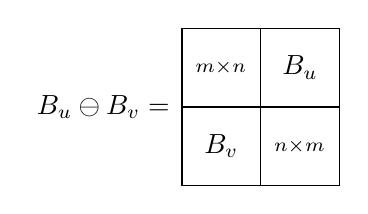
\begin{tikzpicture}
        \node at (-1.5,-0.5) {$B_u\ominus B_v =$};
        \draw[
            step=1.0,xshift=-0.5cm,yshift=0.5cm,
            black,thin
        ] (0,0) grid (2,-2);
        \node at (0,0) {$\blank_{m\times n}$};
        \node at (1,0) {$B_u$};
        \node at (0,-1) {$B_v$};
        \node at (1,-1) {$\cross_{n\times m}$};
    \end{tikzpicture}
\]
where $B_u\in \BPD(u)$ and $B_v\in \BPD(v)$.
Here $\blank_{m\times n}$ is an $m\times n$ grid of $\blank$ tiles, and $\cross_{n\times m}$ is an $n\times m$ grid of $\cross$ tiles.
\end{proposition}

We refer to $B_u\ominus B_v$ as the \textit{skew sum} of $B_u$ and $B_v$, which also makes sense to define for diagrams that are not bumpless pipe dreams.
We remark that Proposition \ref{prop:skew_BPD} is proven in \cite{HPS22} for reduced bumpless pipe dreams, with the generalization here essentially following the same argument.
To help with our proof of Proposition \ref{prop:skew_BPD}, we first prove the following lemma:

\begin{lemma}
\label{lem:skew_reduce}
    Let $B_u\in \BPD(u)$ and $B_v\in \BPD(v)$.
    Then \[
        \reduce(B_u\ominus B_v)
        = \reduce(B_u)\ominus \reduce(B_v).
    \]
\end{lemma}

\begin{proof}
    Write $B = B_u\ominus B_v$.
    Observe that pipes in $B$ of the form $y\to x$ where $x\in [m]$ only pass through the regions $B_u$ and $\cross_{n\times m}$.
    Similarly, the pipes of the form $y'\to x'$ where $x'\in [m+1,m+n] := \{m+1,\dots,m+n\}$ only pass through the regions $B_v$ and $\cross_{n\times m}$.
    Thus each of the $mn$ pairs of pipes $y\to x$ and $y'\to x'$ notated as above cross at one of the $mn$ $\cross$'s in the region $\cross_{n\times m}$, and this is the only time this pair crosses in $B$.
    In particular, any pipes in $B$ that cross more than once must do so internally to either of the regions $B_u$ or $B_v$.
    
    These observations remain unchanged no matter how many $\cross$'s in $B_u$ or $B_v$ we change into $\bump$'s (though the specific pipes passing through each $\cross$ in $\cross_{n\times m}$ may change).
    Hence when passing to $\reduce(B)$, we resolve all of the double crossings in $B_v$ while keeping the region $\cross_{n\times m}$ unchanged, then resolve the double crossings in $B_u$.
    The desired decomposition then follows.
\end{proof}

\begin{figure}
\begin{tikzpicture}[scale=0.5]
    \drawBPD{0}{2}{5}{
        0,0,4,2,2,
        0,0,1,4,2,
        0,4,3,3,2,
        4,3,3,5,4,
        1,1,1,4,3
    }
    \node at (5.5,0) {$\ominus$};
    \begin{scope}[shift = {(0,0.5)}]
    \drawBPD{7}{1}{4}{
        0,0,4,2,
        0,4,3,2,
        4,3,5,4,
        1,1,4,3
    }
    \end{scope}
    \node at (11.5,0) {$=$};
    \drawBPD{13}{4}{9}{
        0,0,0,0,0,0,4,2,2,
        0,0,0,0,0,0,1,4,2,
        0,0,0,0,0,4,3,3,2,
        0,0,0,0,4,3,3,5,4,
        0,0,0,0,1,1,1,4,3,
        0,0,4,2,3,3,3,3,3,
        0,4,3,2,3,3,3,3,3,
        4,3,5,4,3,3,3,3,3,
        1,1,4,3,3,3,3,3,3
    }
    \draw (16.5,4.5) -- (16.5,-4.5);
    \draw[thick] (12.5,-0.5) -- (21.5,-0.5);
    
    \begin{scope}[shift = {(0,-10)}]
    \drawBPDwithL{0}{2}{5}{
        0,0,4,2,2,
        0,0,1,4,2,
        0,4,3,6,2,
        4,3,3,5,4,
        1,1,1,4,3
    }{1/3,2/2,3/1,4/5,5/4}
    \node at (5.75,0) {$\ominus$};
    \begin{scope}[shift = {(0,0.5)}]
    \drawBPDwithL{7}{1}{4}{
        0,0,4,2,
        0,4,6,2,
        4,3,5,4,
        1,1,4,3
    }{1/2,2/1,3/4,4/3}
    \end{scope}
    \node at (11.75,0) {$=$};
    \drawBPDwithL{13}{4}{9}{
        0,0,0,0,0,0,4,2,2,
        0,0,0,0,0,0,1,4,2,
        0,0,0,0,0,4,3,6,2,
        0,0,0,0,4,3,3,5,4,
        0,0,0,0,1,1,1,4,3,
        0,0,4,2,3,3,3,3,3,
        0,4,6,2,3,3,3,3,3,
        4,3,5,4,3,3,3,3,3,
        1,1,4,3,3,3,3,3,3
    }{1/7,2/6,3/5,4/9,5/8,6/2,7/1,8/4,9/3}
    \draw (16.5,4.5) -- (16.5,-4.5);
    \draw[thick] (12.5,-0.5) -- (21.5,-0.5);
    \end{scope}
\end{tikzpicture}

\caption{
    Top: The skew sum of two bumpless pipe dreams $B_u\in \BPD(2143)$ and $B_v\in \BPD(32154)$.
    Bottom: The skew sum of $\reduce(B_u)$ and $\reduce(B_v)$.
    Notice that $\reduce(B_u\ominus B_v) = \reduce(B_u)\ominus \reduce(B_v)$.
}
\label{}
\end{figure}



\begin{proof}[Proof of Proposition \ref{prop:skew_BPD}]
Let $B\in \BPD(u\ominus v)$.
If $y\to x$ is a pipe in $\reduce(B)$ with $x\in [m]$, then $y = u\ominus v(x) = u(x)+n \in [n+1,m+n]$, so $y\to x$ must stay within in the region $[m+n]\times[n+1,n+m]$.
Likewise, if $y'\to x'$ is a pipe in $\reduce(B)$ with $x'\in [m+1,m+n]$, then $y' = u\ominus v(x') = v(x'-m) \in [n]$, so $y'\to x'$ must stay in the region $[m+1,m+n]\times [m+n]$.
It follows that $\reduce(B)_{i,j} = \blank$, and hence $B_{i,j} = \blank$, for all $(i,j)\in [m]\times [n]$.

Furthermore, if $y\to x$ and $y'\to x'$ is a pair of pipes as above, then we saw $x < x'$ while $y > y'$, so $y\to x$ and $y'\to x'$ must cross in $\reduce(B)$.
This can only happen in the region $[m+1,m+n]\times [n+1,m+n]$.
Since there are $mn$ such pairs of pipes, we must have that $\reduce(B)_{i,j} = \cross$, and hence $B_{i,j} = \cross$, for all $(i,j)\in [m+1,m+n]\times [n+1,m+n]$.

It follows that $B = B_1\ominus B_2$ for some bumpless pipe dreams $B_1$ and $B_2$.
By Lemma \ref{lem:skew_reduce}, $\reduce(B) = \reduce(B_1)\ominus \reduce(B_2)$.
Since $B$ has permutation $u\ominus v$, it follows that $B_1$ has permutation $u$ and $B_2$ has permutation $v$.
Hence $B_1\in \BPD(u)$ and $B_2\in \BPD(v)$.

Conversely, suppose that $B = B_u\ominus B_v$ for some $B_u\in \BPD(u)$ and $B_v\in \BPD(v)$.
Then $\reduce(B) = \reduce(B_u)\ominus \reduce(B_v)$ by Lemma \ref{lem:skew_reduce}, from which it is clear that $B$ has permutation $u\ominus v$.
\end{proof}



Let $B = B_u\ominus B_v\in \BPD(u\ominus v)$.
Notice that the contribution of $B$ in Equation \ref{eq:groth} for the $\beta$-Grothendieck polynomial $\fk G_{u\ominus v}^{(\beta)}(x_1,\dots,x_{m+n-1})$ can be computed as
\begin{align*}
    &\beta^{-\ell(u\ominus v)}
    \bigg(
        \prod_{B(\smallblank)} \beta x_i
    \bigg)
    \bigg(
        \prod_{B(\smalljelbow)} (1+\beta x_i)
    \bigg)\\
    &\hspace{8em}=
    \beta^{-mn-\ell(u)-\ell(v)}
    \bigg(
        \prod_{\smallblank_{m\times n}} \beta x_i
        \prod_{B_u(\smallblank)} \beta x_i
        \prod_{B_v(\smallblank)} \beta x_{m+i}
    \bigg)\\
    &\hspace{14em}
    \bigg(
        \prod_{B_u(\smalljelbow)} (1+\beta x_i)
        \prod_{B_v(\smalljelbow)} (1+\beta x_{m+i})
    \bigg)
    \\
    &\hspace{8em}=
    x_1^nx_2^n\cdots x_m^n\, \beta^{-\ell(u)}
    \bigg(
        \prod_{B_u(\smallblank)} \beta x_i
        \prod_{B_u(\smalljelbow)} (1+\beta x_i)
    \bigg)
    \\
    &\hspace{14em}
    \beta^{-\ell(v)}
    \bigg(
        \prod_{B_v(\smallblank)} \beta x_{m+i}
        \prod_{B_v(\smalljelbow)} (1+\beta x_{m+i})
    \bigg).
\end{align*}
This is $x_1^nx_2^n\cdots x_m^n$ times the product of the contribution of $B_u$ in $\fk G_u^{(\beta)}(x_1,\dots,x_{m-1})$ and the contribution of $B_v$ in $\fk G_v^{(\beta)}(x_{m+1},\dots,x_{m+n-1})$ with the indices shifted as indicated.
Combining this with Proposition \ref{prop:skew_BPD} gives the following multiplicative formulae for skew sums:

\begin{proposition}
\label{prop:skew_formulae}
    Let $u\in S_m$ and $v\in S_n$.
    Then \[
        \fk G_{u\ominus v}^{(\beta)}(x_1,\dots,x_{m+n-1})
        = x_1^nx_2^n\cdots x_m^n
        \fk G_u^{(\beta)}(x_1,\dots,x_{m-1})
        \fk G_v^{(\beta)}(x_{m+1},\dots,x_{m+n-1})
    \]
    In particular, $\nu^{(\beta)}_{u\ominus v} = \nu^{(\beta)}_u \nu^{(\beta)}_v$ and 
    $c^{(\beta)}_{u\ominus v} = c^{(\beta)}_u c^{(\beta)}_v$.
\end{proposition}

\begin{proof}
It remains to show that $c^{(\beta)}_{u\ominus v} = c^{(\beta)}_u c^{(\beta)}_v$.
The subwords of $u\ominus v$ are themselves of the form $u'\ominus_n v'$ for subwords $u'\sseq u$ and $v'\sseq v$,
where by $u'\ominus_n v'$ we mean the word $(u'(1)+n)\dots (u'(\abs*{u'})+n)\ v'(1)\cdots v'(\abs*{v'})$.
It is clear that $\perm(u'\ominus_n v') = \perm(u')\ominus \perm(v')$.
By applying inclusion-exclusion, we then get \begin{align*}
    c^{(\beta)}_{u\ominus v}
    &= \sum_{u'\ominus_n v'\, \sseq\, u\ominus v}
    (-1)^{\abs*{u\ominus v} - \abs*{u'\ominus v'}}
    \nu^{(\beta)}_{\perm(u'\ominus v')} \\
    &= \sum_{u'\sseq u} \sum_{v'\sseq v}
    (-1)^{\abs*{u} + \abs*{v} - \abs*{u'} - \abs*{v'}}
    \nu^{(\beta)}_{\perm(u')\ominus \perm(v')} \\
    &= \sum_{u'\sseq u} \sum_{v'\sseq v}
    (-1)^{\abs*{u}-\abs*{u'}} (-1)^{\abs*{v}-\abs*{v'}}  
    \nu^{(\beta)}_{\perm(u')} \nu^{(\beta)}_{\perm(v')} \\
    &= \Big(
        \sum_{u'\sseq u}
        (-1)^{\abs*{u}-\abs*{u'}} \nu^{(\beta)}_{\perm(u')}
    \Big)
    \Big(
        \sum_{v'\sseq v}
        (-1)^{\abs*{v}-\abs*{v'}} \nu^{(\beta)}_{\perm(v')}
    \Big) \\
    &= c^{(\beta)}_u c^{(\beta)}_v. \qedhere
\end{align*}
\end{proof}




